\documentclass[conference]{IEEEtran}

\usepackage[T1]{fontenc}
\usepackage[utf8]{inputenc}
\usepackage{cite}
\usepackage{graphicx}
\usepackage{array}
\usepackage{booktabs}
\usepackage{tabularx}
\usepackage{url}
\usepackage{hyperref}
\usepackage{balance}
\usepackage{booktabs}
\usepackage{tabularx}
\usepackage{array}
\usepackage{capt-of}
\usepackage{makecell}
\usepackage{cuted}
\usepackage{capt-of}

\hypersetup{
    colorlinks=true,
    linkcolor=black,
    citecolor=black,
    urlcolor=blue
}

\newcolumntype{L}[1]{>{\raggedright\arraybackslash}p{#1}}

\newcommand{\safeimage}[2]{%
    \IfFileExists{#1}{%
        \includegraphics[width=\linewidth]{#1}%
    }{%
        \fbox{%
            \parbox[c][4.0cm][c]{0.95\linewidth}{%
                \centering
                Screenshot placeholder\\[4pt]
                #2\\[4pt]
                {\ttfamily\small\detokenize{#1}}
            }%
        }%
    }%
}

\title{A TCP Socket-Based Multi-User Messaging System with a Graphical Client and Reliable File Transfer}

\author{
	\begin{minipage}[t]{0.30\textwidth}
		\centering
		Li Haolin\\
		The Education University of Hong Kong\\
		Email: s1153657@s.eduhk.hk
	\end{minipage}
	\hfill
	\begin{minipage}[t]{0.30\textwidth}
		\centering
		Lam Chun Kit\\
		The Education University of Hong Kong\\
		Email: s1154051@s.eduhk.hk
	\end{minipage}
	\hfill
	\begin{minipage}[t]{0.30\textwidth}
		\centering
		Liu Chenghao\\
		The Education University of Hong Kong\\
		Email: s1153655@s.eduhk.hk
	\end{minipage}
}

\begin{document}
	
	\maketitle

\begin{abstract}
	This paper presents the design and implementation of a TCP socket-based multi-user messaging system in Python. The system follows a client-server architecture and supports the core functions of a message application, including authentication, friend list management, direct and broadcast messaging, text-file delivery, inbox operations, and acknowledgement generation. Server-side data, including user records, friend lists, messages, and files, are persistently maintained in JSON format, while communication is handled through a lightweight custom application-layer protocol.
	
	To extend the baseline project requirements, the system incorporates a Tkinter-based graphical client, online/offline friend status display, and an enhanced file-transfer mechanism with chunked transmission, SHA-256 integrity verification, optional compression, and progress-bar feedback. These additions improve both usability and transfer robustness while preserving a simple and readable implementation structure. The final system provides a compact but complete demonstration of socket programming, protocol design, persistent messaging services, and practical reliability enhancements in a student-level network application.
\end{abstract}


\section{Introduction}

Socket programming is a fundamental topic in internetworking because it links transport-layer communication with the design of application-layer protocols and client-server systems. To explore these concepts in a practical setting, this project implements a TCP socket-based multi-user messaging system in Python. The system adopts a client-server architecture and a lightweight custom text-based protocol to support user communication, persistent message storage, and file delivery over the network.

Beyond the baseline functions required by the project specification, the final system extends the messaging platform with user registration, online/offline friend status display, a Tkinter-based graphical client, and a more reliable file-transfer workflow based on chunked transmission, SHA-256 integrity verification, optional compression, and progress feedback. These enhancements improve both usability and transfer robustness while keeping the implementation compact and easy to inspect. The remainder of this paper describes the system architecture, details the steps required to run the client and server applications, and presents the protocol specification used in the implementation.


\section{System Overview}

\subsection{Project Structure}
The implementation is divided into a set of modules for configuration, protocol handling, storage, server-side control, and client-side interaction. Table~\ref{tab:project-structure} summarizes the role of each main component.

\begin{table}[!t]
	\caption{Main Project Components}
	\label{tab:project-structure}
	\centering
	\footnotesize
	\renewcommand{\arraystretch}{1.15}
	\begin{tabularx}{\columnwidth}{
			>{\raggedright\arraybackslash}p{0.34\columnwidth}
			>{\raggedright\arraybackslash}p{0.60\columnwidth}
		}
		\toprule
		\textbf{File / Directory} & \textbf{Main Responsibility} \\
		\midrule
		\texttt{src/config.py} &
		Defines network parameters and transfer-related settings, such as host, port, buffer size, chunk size, and compression threshold. \\
		
		\texttt{src/protocol.py} &
		Implements request/response formatting, field escaping and restoration, and helper functions for file-transfer processing. \\
		
		\texttt{src/storage.py} &
		Handles persistent data management, including user records, friend lists, inbox items, file records, and acknowledgement entries. \\
		
		\texttt{src/server.py} &
		Implements the core server logic, including socket setup, client-session handling, command validation, online-status tracking, and transfer reassembly. \\
		
		\texttt{src/client.py} &
		Provides a basic command-line client for compatibility testing and simple manual interaction with the server. \\
		
		\texttt{src/gui\_client.py} &
		Provides the main Tkinter-based graphical client for login, messaging, file transfer, inbox access, and transfer progress display. \\
		
		\texttt{data/} &
		Stores persistent JSON data files used by the server, including default user information and server-side messaging data. \\
		
		\texttt{text\_files/} &
		Contains sample text files used for file-transfer testing and demonstration scenarios. \\
		\bottomrule
	\end{tabularx}
\end{table}


\subsection{Design Goals}
The system design is guided by the following principles:
\begin{itemize}
	\item \textbf{Functional completeness:} The implementation should fully cover the baseline project requirements through a coherent client-server architecture for messaging, file transfer, inbox operations, and acknowledgement handling.
	
	\item \textbf{Protocol and storage clarity:} The application-layer protocol and storage model should remain lightweight and inspectable, so that command formats, validation logic, and persistent data organization can be clearly understood and verified.
	
	\item \textbf{Usability for demonstration:} The client interface should support reliable demonstration and convenient interaction, with the Tkinter GUI acting as the primary interface and the CLI client preserved for compatibility and manual testing.
	
	\item \textbf{Practical enhancement:} The system should incorporate meaningful extensions beyond the baseline specification, particularly in transfer reliability and usability, while preserving readability, modularity, and maintainability.
\end{itemize}

\vspace*{0.5\baselineskip}
\section{Architecture and Implementation}
\subsection{Server Side}
The server is implemented in \texttt{src/server.py} as the central control component of the system. It uses Python TCP sockets to accept client connections and creates one worker thread for each connected client, allowing multiple users to interact with the messaging service concurrently. For each request, the server parses the command, validates the sender identity and parameters, applies the required business logic, updates persistent data through the storage layer, and returns a compact success or error response to the client.

In addition to handling the baseline messaging workflow, the server is responsible for maintaining online session state and coordinating the enhanced file-transfer process. Online users are tracked through an in-memory connection map, which allows the system to support reconnect behavior and provide explicit online/offline status information to the GUI client. For chunked file transfer, the server also manages temporary transfer state, receives incoming chunks, performs reassembly and verification, and converts the final payload into a normal stored inbox item after successful validation.

\subsection{Storage Layer}
Persistent storage is managed through JSON files located under \texttt{data/}, primarily \texttt{default\_users.json} and \texttt{server\_data.json}. This layer stores user records, friendship relationships, messages, files, and acknowledgement entries in a human-readable format. Such a design is intentionally lightweight and inspectable, making the stored system state easy to verify during development, testing, and project demonstration.

The storage model is organized around logical messaging data rather than transport-specific representations. In particular, even when a file is transmitted using compression and chunking, the final saved content is restored to normal text form before being written into persistent storage. This keeps the transport mechanism separated from the long-term data representation and avoids introducing unnecessary complexity into the persistence layer.

\subsection{Client Side}
The project provides two client interfaces with different purposes. The command-line client in \texttt{src/client.py} preserves the original menu-driven interaction model and serves mainly as a compatibility and manual testing interface. It is useful for verifying baseline protocol behavior without relying on graphical components.

The primary demonstration interface is the Tkinter-based GUI client in \texttt{src/gui\_client.py}. It supports the main user workflow, including login, registration, friend-list operations, online/offline status refresh, direct messaging, broadcast messaging, file transfer, inbox access, and reconnect handling. In addition, the GUI exposes the enhanced transfer workflow more clearly by providing visible status updates and progress-bar feedback during large file transmission. This makes the client more suitable for live presentation while preserving consistency with the same server-side protocol and storage model.

\subsection{Current Transfer Settings}
The current implementation uses the configuration values shown in Table~\ref{tab:transfer-settings}.

\begin{center}
	\footnotesize
	\captionof{table}{Current Transfer Settings}
	\label{tab:transfer-settings}
	\renewcommand{\arraystretch}{1.15}
	\begin{tabularx}{\columnwidth}{
			>{\raggedright\arraybackslash}p{0.42\columnwidth}
			>{\raggedright\arraybackslash}p{0.20\columnwidth}
			>{\raggedright\arraybackslash}p{0.30\columnwidth}
		}
		\toprule
		\textbf{Parameter} & \textbf{Value} & \textbf{Description} \\
		\midrule
		Server host & \texttt{0.0.0.0} & Server bind address \\
		Client host & \texttt{127.0.0.1} & Default client connection target \\
		Port & \texttt{12345} & TCP service port \\
		Socket buffer size & \texttt{1024} & Receive/send buffer size used by the socket logic \\
		Transfer chunk size & \texttt{700} & Maximum payload size of each transfer chunk \\
		Compression threshold & \texttt{256} bytes & Minimum payload size for applying compression \\
		\bottomrule
	\end{tabularx}
\end{center}

\vspace{0.65\baselineskip}
\section{Detailed Running Instructions}
This section is based on the actual current project structure and was verified in an environment with Python~3.13.3. The project uses only Python standard-library modules.

\subsection{Environment and Files}
Before running the project, confirm the following items:
\begin{itemize}
\item Python 3 is installed and available as \texttt{python3}.
\item The project root contains \texttt{src/}, \texttt{data/}, \texttt{docs/}, and \texttt{text\_files/}.
\end{itemize}

\subsection{Start the Server}
Open a terminal in the project root and run:
\begin{verbatim}
python3 src/server.py
\end{verbatim}
The server listens on port \texttt{12345}. Keep this terminal open while using any client.

\subsection{Start the GUI Client}
Open another terminal in the project root and run:
\begin{verbatim}
python3 src/gui_client.py
\end{verbatim}
For a two-user demonstration, open a second GUI client in another terminal and log in as a different user.

\subsection{Default Accounts and Registration}
The project already includes 10 default users as required in \texttt{data/default\_users.json}. New accounts can also be created from the GUI login window with the Register function. 

\subsection{Practical Demo Flow}
The most reliable demonstration sequence is:
\begin{enumerate}
\item start the server;
\item open two GUI clients;
\item log in as two different users;
\item add each other as friends if needed;
\item refresh the friend list and friend status;
\item send a normal text message;
\item send a broadcast message;
\item send a small text file such as \texttt{text\_files/sample1.txt};
\item send a large text file such as \texttt{text\_files/sample3.txt} to trigger compression and multiple chunks;
\item open the receiver inbox and read the incoming items.
\end{enumerate}

\subsection{Role of the CLI Client}
The CLI client still exists and can be started with:
\begin{verbatim}
python3 src/client.py
\end{verbatim}
Its role is compatibility and simple manual testing. The final project demonstration should focus on the GUI because the progress bar and chunked transfer workflow are implemented there with the least code disruption.

\vspace{0.7\baselineskip}
\section{Protocol Specification}
\subsection{General Message Format}
The implementation uses a lightweight text-based application-layer protocol over TCP. Each request begins with a command name followed by one or more parameters separated by the vertical bar character \texttt{|}. For commands that involve multiple recipients, user IDs are encoded as a comma-separated list inside a single field. To preserve protocol compatibility, free-text content is escaped before transmission and restored after parsing by helper functions in \texttt{src/protocol.py}.

Most server replies follow a uniform reply structure:
\begin{quote}
	\texttt{OK|COMMAND|message}
\end{quote}
for successful processing, and
\begin{quote}
	\texttt{ERROR|COMMAND|message}
\end{quote}
for invalid requests or failed validation. Some commands, such as \texttt{READ\_ITEM}, return additional structured fields after the command name in order to carry message or file metadata together with the item content. This design keeps the protocol easy to inspect while still supporting the full messaging workflow.

\subsection{Core Commands}
Table~\ref{tab:core-commands} summarizes the main commands used in the baseline messaging workflow.

\begin{strip}
	\centering
	\scriptsize
	\captionof{table}{Core Protocol Commands}
	\label{tab:core-commands}
	\renewcommand{\arraystretch}{0.96}
	\setlength{\tabcolsep}{2.6pt}
	
	\newcommand{\codecell}[1]{\makecell[l]{\scriptsize\texttt{#1}}}
	\newcommand{\twolinecode}[2]{\makecell[l]{\scriptsize\texttt{#1}\\[-1.5pt]\scriptsize\texttt{#2}}}
	\newcommand{\threelinecode}[3]{\makecell[l]{\scriptsize\texttt{#1}\\[-1.5pt]\scriptsize\texttt{#2}\\[-1.5pt]\scriptsize\texttt{#3}}}
	
	\begin{tabularx}{\textwidth}{
			>{\raggedright\arraybackslash}p{0.15\textwidth}
			>{\raggedright\arraybackslash}p{0.27\textwidth}
			>{\raggedright\arraybackslash}X
		}
		\toprule
		\textbf{Command} & \textbf{Request Format} & \textbf{Main Rules / Behavior} \\
		\midrule
		
		\codecell{LOGIN} &
		\codecell{LOGIN|user\_id|password} &
		Authenticates an existing user. The account must exist and the password must match. A successful request returns a standard \texttt{OK} reply and marks the user as logged in. \\
		
		\codecell{REGISTER} &
		\codecell{REGISTER|user\_id|password} &
		Creates a new account. The user ID must contain lowercase letters or digits only, must not already exist, and the password must be non-empty. \\
		
		\codecell{VIEW\_FRIENDS} &
		\codecell{VIEW\_FRIENDS|user\_id} &
		Returns the caller's friend list. The requester must already be logged in and may only request its own data. If no friends exist, the server returns \texttt{NO\_FRIENDS}. \\
		
		\twolinecode{VIEW\_FRIENDS\_}{STATUS} &
		\twolinecode{VIEW\_FRIENDS\_STATUS}{|user\_id} &
		Returns the caller's friend list together with online/offline state derived from current server-side session tracking. The same identity checks as \texttt{VIEW\_FRIENDS} apply. \\
		
		\codecell{ADD\_FRIEND} &
		\codecell{ADD\_FRIEND|user\_id|friend\_id} &
		Adds an existing user to the caller's friend list. Both users must exist, self-addition is rejected, and duplicate friendship is not allowed. \\
		
		\codecell{DELETE\_FRIEND} &
		\twolinecode{DELETE\_FRIEND}{|user\_id|friend\_id} &
		Removes an existing friend from the caller's friend list. The requester must be logged in and the target must already be present in the current friend list. \\
		
		\codecell{SEND\_MESSAGE} &
		\twolinecode{SEND\_MESSAGE}{|sender|r1,r2|content} &
		Sends a text message to one or more valid friends. The sender must be logged in, recipients must be existing friends, and self-sending is rejected. Multi-line content is supported after escaping. \\
		
		\codecell{BROADCAST} &
		\codecell{BROADCAST|sender|content} &
		Sends the same message to all friends of the sender. The sender must be logged in and must already have at least one friend. \\
		
		\codecell{SEND\_FILE} &
		\threelinecode{SEND\_FILE}{|sender|r1,r2|}{file\_name|file\_content} &
		Sends a text file to one or more valid friends. The sender must be logged in, recipients must be friends, the file must use the \texttt{.txt} extension, and the content must not be empty. \\
		
		\codecell{LIST\_INBOX} &
		\codecell{LIST\_INBOX|user\_id} &
		Returns a summary view of the caller's inbox. The requester must be logged in and may only access its own inbox. \\
		
		\codecell{READ\_ITEM} &
		\twolinecode{READ\_ITEM}{|user\_id|item\_number} &
		Returns the full content of the selected inbox item together with its metadata. The item number must be a valid positive index. Reading a direct message or file also triggers acknowledgement generation for the original sender. \\
		
		\codecell{DELETE\_ITEM} &
		\twolinecode{DELETE\_ITEM}{|user\_id|item\_number} &
		Deletes the selected inbox item. The same index validation rules as \texttt{READ\_ITEM} apply. \\
		
		\codecell{LOGOUT} &
		\codecell{LOGOUT} &
		Ends the current authenticated session and returns a standard logout confirmation reply. This command is valid only after login. \\
		
		\bottomrule
	\end{tabularx}
\end{strip}


\subsection{Acknowledgement Behavior}
Acknowledgement is implemented as a normal inbox item generated by the server. When a user reads a direct message or file item, the server creates an acknowledgement entry in the original sender's inbox indicating that the item has been read. Broadcast items and acknowledgement items do not trigger further acknowledgement generation, which prevents recursive acknowledgement chains and keeps the inbox behavior predictable.

\subsection{Chunked Transfer Extension}
The final version extends the baseline file-transfer workflow with two additional protocol commands dedicated to GUI-based large-file delivery: \texttt{TRANSFER\_START} and \texttt{TRANSFER\_CHUNK}. The \texttt{TRANSFER\_START} request carries transfer metadata, including the sender identity, recipient list, transfer identifier, file name, total chunk count, compression flag, and checksum information. The \texttt{TRANSFER\_CHUNK} request carries the indexed payload chunks associated with that transfer. Together, these two commands allow the server to validate transfer metadata, accept and track chunked input, reject invalid or duplicate chunks, reconstruct the original payload, verify integrity, perform decompression when required, and then save the final file through the normal inbox and storage path.


The transfer sequence in the current implementation is:
\begin{enumerate}
\item read the text file in the GUI client;
\item encode the file content as UTF-8 text;
\item compress it with \texttt{zlib} when the content size is at least \texttt{256} bytes~\cite{python_zlib};
\item compute a SHA-256 checksum on the transfer bytes~\cite{python_hashlib};
\item Base64-encode the transfer bytes;
\item split the Base64 payload into chunks of up to \texttt{700} characters;
\item send one \texttt{TRANSFER\_START} request and then all \texttt{TRANSFER\_CHUNK} requests;
\item reassemble the chunks on the server, verify checksum, decompress if needed, decode the original text, and save the final file item.
\end{enumerate}


\vspace{0.7\baselineskip}
\section{Key Features and Enhancements}

\subsection{Baseline Functional Coverage}
The implemented system covers the full baseline workflow required for the messaging application project:
\begin{itemize}
	\item user login and logout;
	\item friend-list viewing, addition, and deletion;
	\item direct message sending to one or more friends;
	\item broadcast messaging to all friends;
	\item text-file sending;
	\item inbox listing, item reading, and item deletion;
	\item acknowledgement generation after a message or file is read;
	\item persistent server-side storage of user data, friend lists, messages, and files;
	\item support for the default set of preconfigured users required at server startup.
\end{itemize}

\subsection{Project Highlights}
Beyond the baseline specification, the final version introduces several enhancements that improve usability, transfer reliability, and overall system completeness. The main additions are summarized in Table~\ref{tab:enhancements}.

\begin{center}
	\footnotesize
	\captionof{table}{Major Enhancements and Practical Value}
	\label{tab:enhancements}
	\renewcommand{\arraystretch}{1.15}
	\begin{tabularx}{\columnwidth}{
			>{\raggedright\arraybackslash}p{0.36\columnwidth}
			>{\raggedright\arraybackslash}X
		}
		\toprule
		\textbf{Enhancement} & \textbf{Practical Value} \\
		\midrule
		
		User registration &
		Removes dependence on a fully fixed user set and makes the messaging system more complete and flexible for demonstration. \\
		
		GUI client &
		Provides a more accessible and presentation-friendly interface than the CLI workflow, especially for live project demonstration. \\
		
		Friend-status display &
		Exposes online/offline presence using server-side session tracking and makes user interaction more informative. \\
		
		Chunked file transfer (\texttt{TRANSFER\_START}, \texttt{TRANSFER\_CHUNK}) &
		Introduces application-layer segmentation and server-side reassembly for large payload delivery, while also making the transfer workflow more realistic and explainable. \\
		
		Integrity verification (SHA-256) &
		Detects damaged or incomplete transferred data before final storage and improves confidence in the correctness of received file content. \\
		
		Optional compression (\texttt{zlib}) &
		Reduces the size of large payloads before transmission and demonstrates an efficiency-oriented design choice for file delivery. \\
		
		Progress feedback in GUI &
		Provides visible status updates during file sending and makes the transfer process easier to observe, explain, and demonstrate. \\
		
		\bottomrule
	\end{tabularx}
\end{center}

\subsection{Why the Final Enhancements Matter}
The final enhancements are important for both networking demonstration and user experience. Chunked transfer makes the protocol more realistic by showing how large application data can be divided into smaller units and reassembled at the application layer. Integrity verification adds a necessary validation step, ensuring that transferred content is checked before it is accepted and stored. Compression introduces an efficiency-oriented design decision for large payloads and demonstrates that transfer behavior can be adapted according to message size.

From the usability perspective, the GUI client, friend-status display, and progress feedback make the system easier to demonstrate and easier to understand during live testing. Instead of hiding protocol activity behind a command-line workflow, the final version exposes more of the system state and transfer process to the user. As a result, the enhancements do not merely add extra features; they also strengthen the project as a complete and explainable internetworking application.


\section{GUI Design Overview}

The graphical user interface is implemented with Tkinter and serves as the primary client for project demonstration. Compared with the command-line client, the GUI presents the system workflow in a more accessible and observable form, especially for login, friend-list interaction, message sending, file transfer, and inbox access. The interface is intentionally kept simple so that the relationship between user actions and underlying protocol behavior remains easy to explain.

\subsection{Login Window}
The login window provides the entry point to the system. It supports user authentication, new-user registration, and reconnect-related interaction in a compact layout. This design allows the demonstration to begin from a clear authentication stage and makes it easier to show both the baseline login workflow and the registration enhancement introduced in the final version.

\vspace{0.3\baselineskip}
\begin{center}
	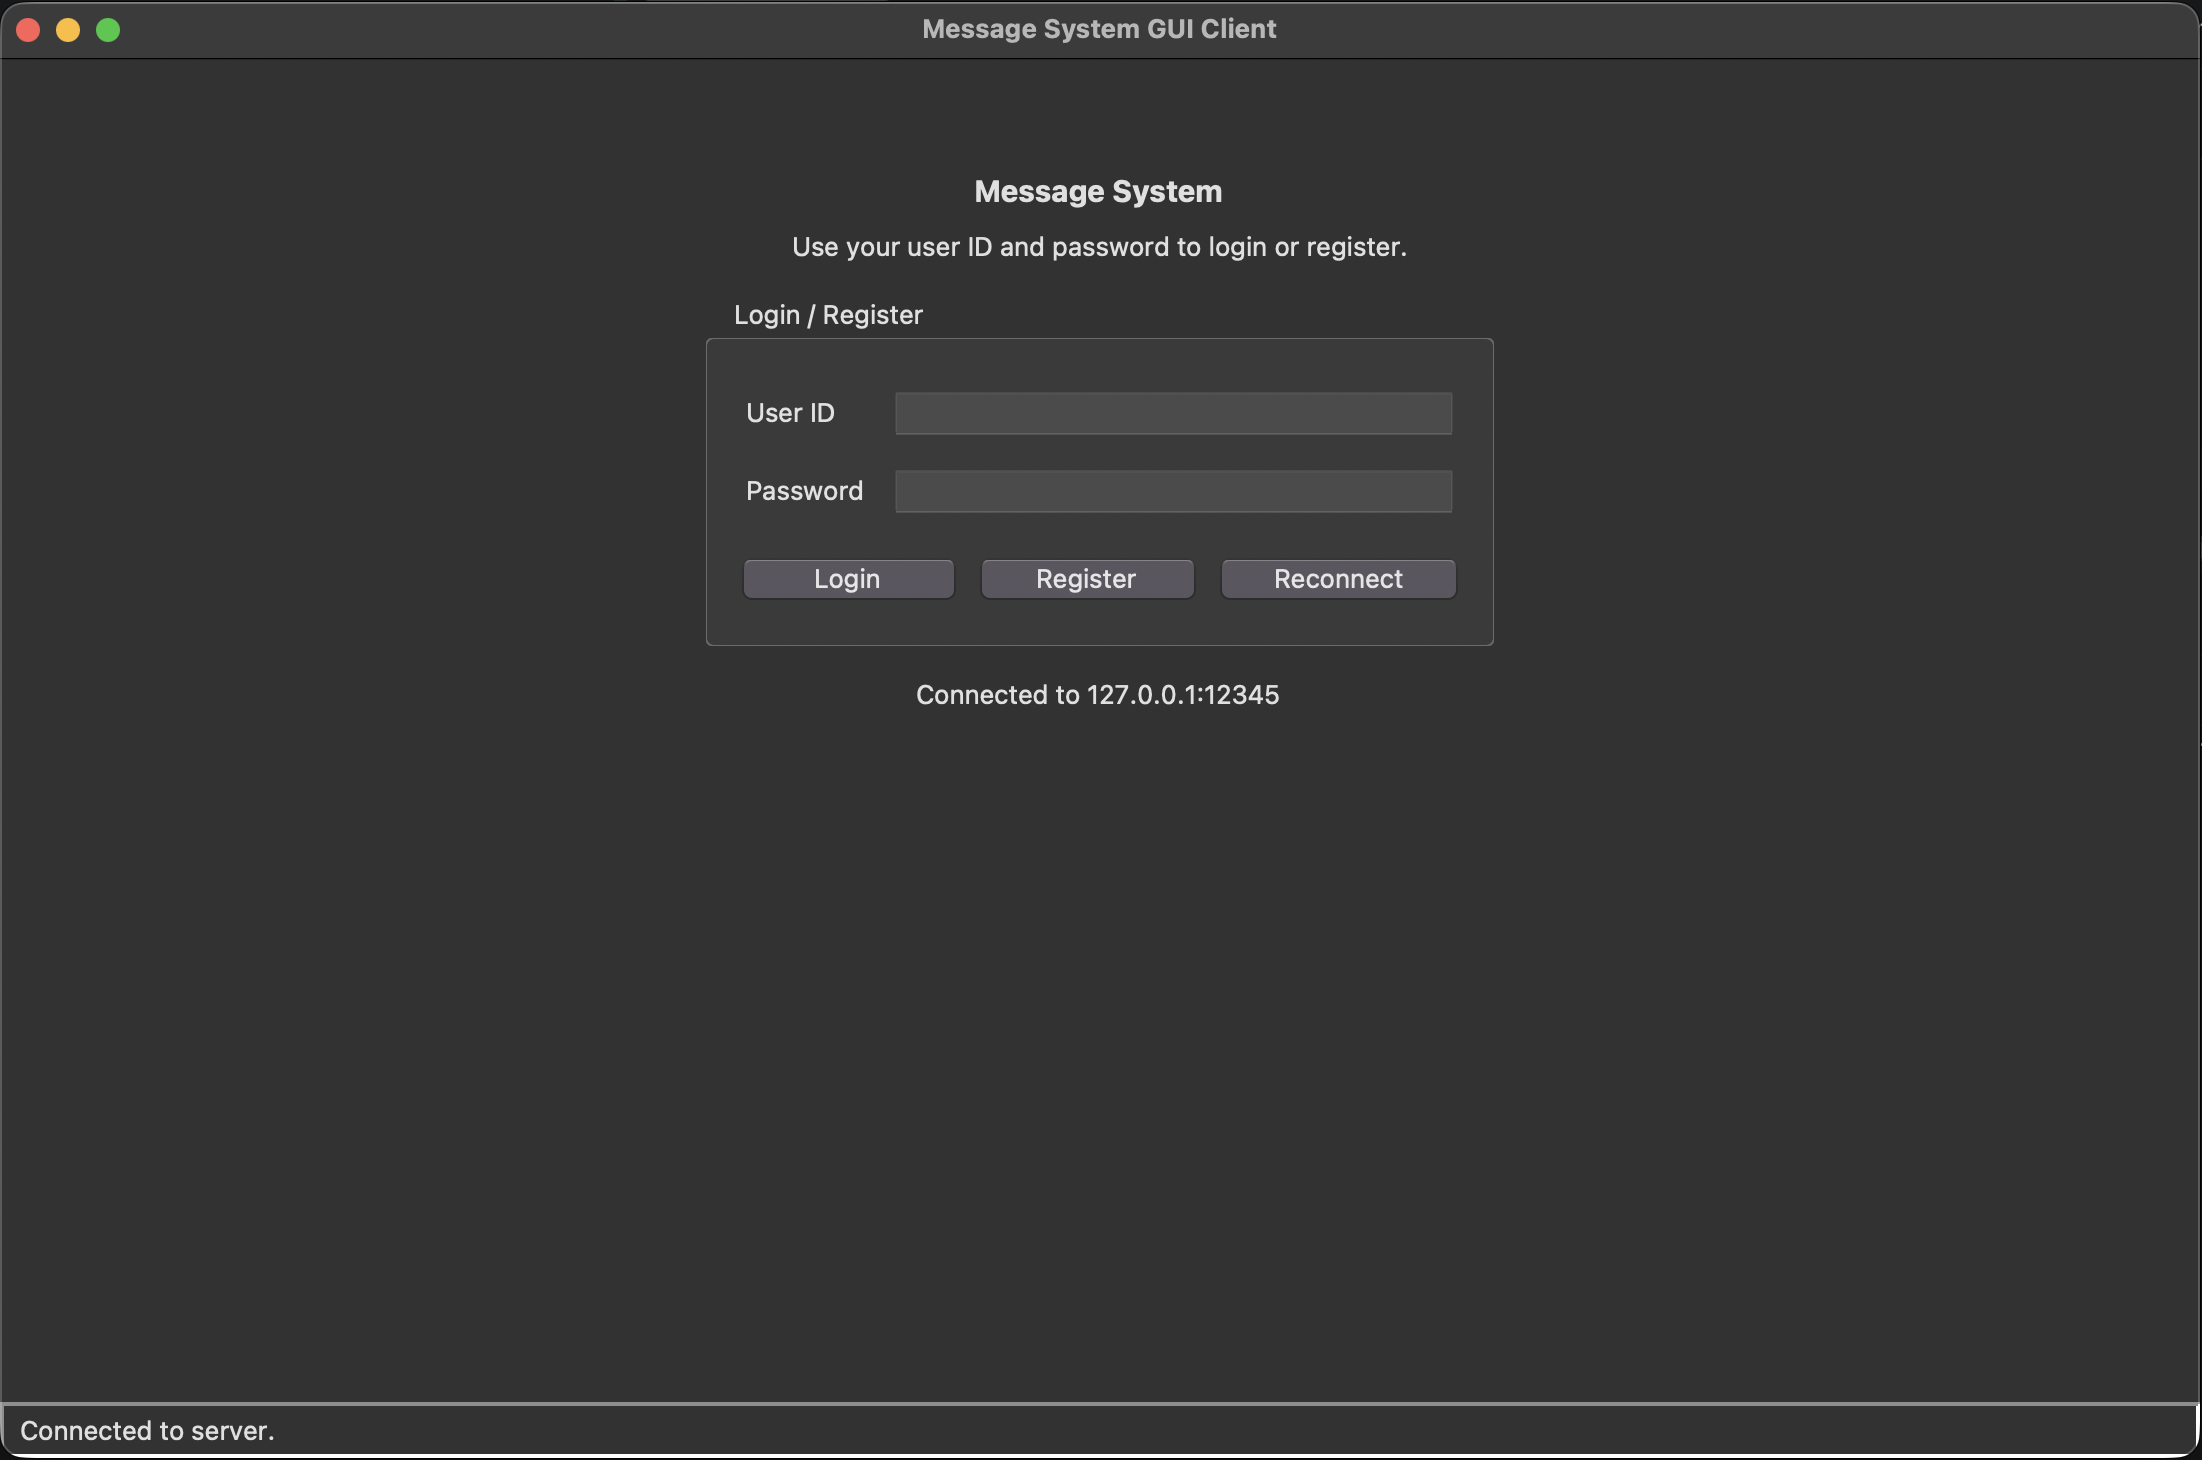
\includegraphics[width=\columnwidth]{figures/gui_login.png}
	\captionof{figure}{Login window of the GUI client.}
	\label{fig:gui-login}
\end{center}
\vspace{0.4\baselineskip}

\subsection{Main Layout}
After successful login, the main window presents the core messaging workflow in a single integrated interface. It shows the current user, connection state, and friend-list area, together with tab-based working panels for direct messaging, broadcast messaging, file transfer, and inbox operations. The file-transfer tab also includes visible status updates and progress feedback, making the enhanced transfer mechanism easier to observe during live demonstration.

\vspace{0.3\baselineskip}
\begin{center}
	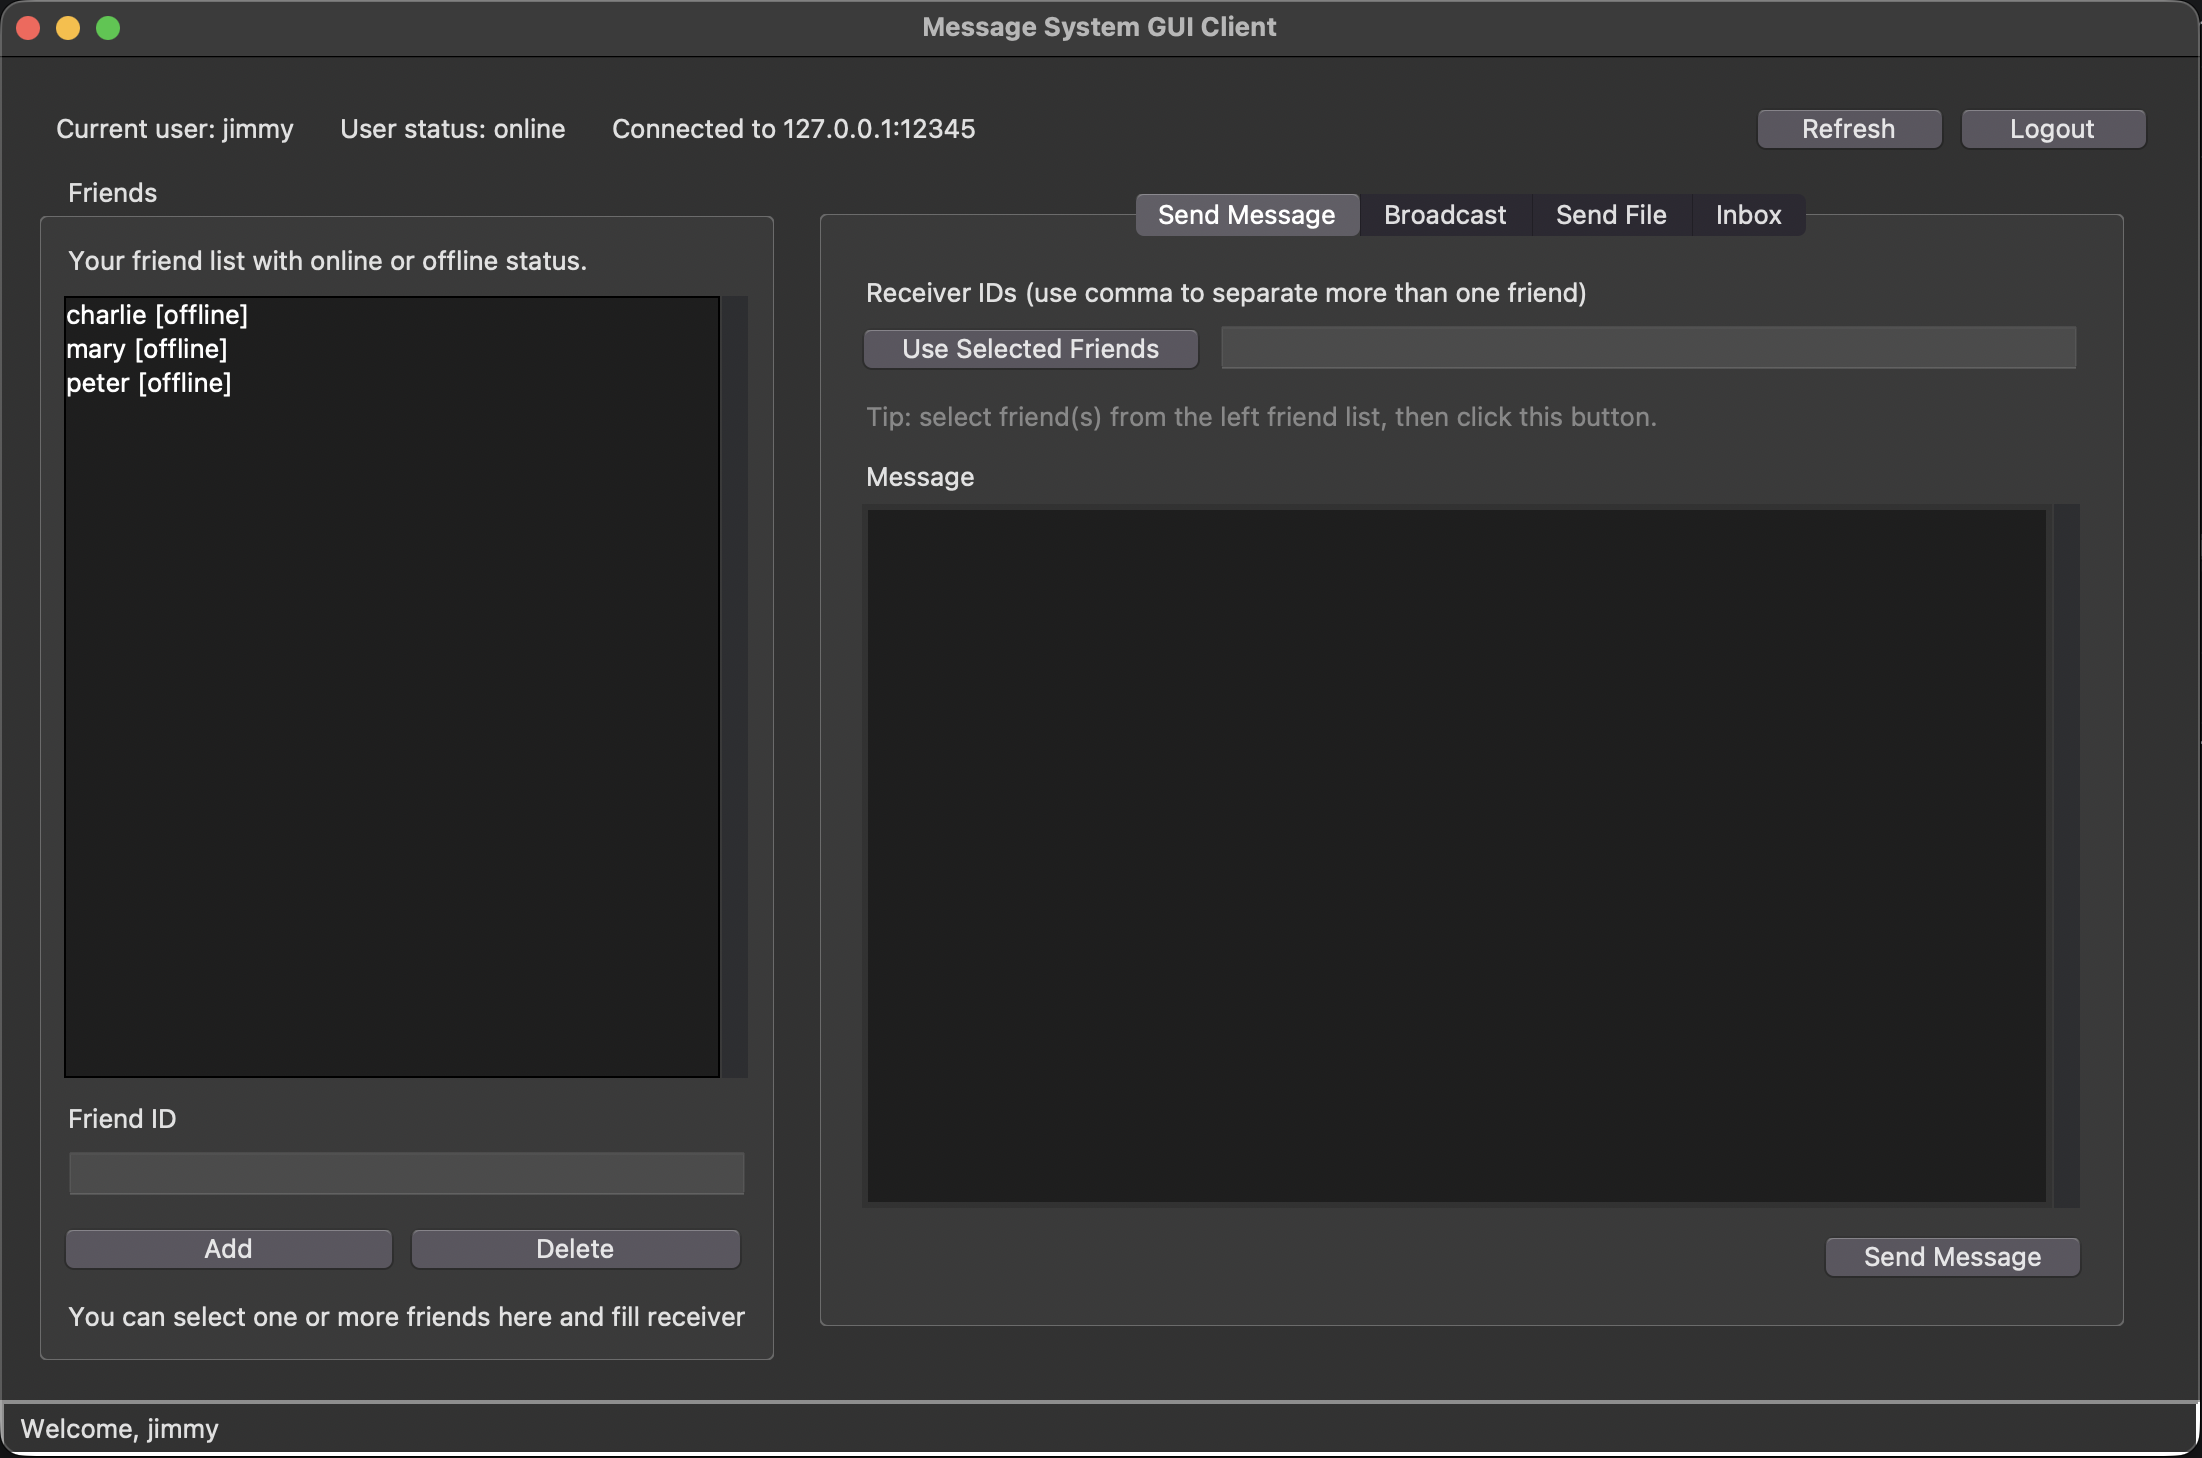
\includegraphics[width=\columnwidth]{figures/gui_main.png}
	\captionof{figure}{Main layout of the GUI client after login.}
	\label{fig:gui-main}
\end{center}
\vspace{0.2\baselineskip}

\vspace{0.5\baselineskip}
\section{Conclusion}
This project presents a complete TCP socket-based multi-user messaging system implemented in Python with a client-server architecture, persistent server-side storage, and a lightweight custom application-layer protocol. The final system satisfies the baseline project requirements, including authentication, friend-list management, direct and broadcast messaging, text-file delivery, inbox operations, and acknowledgement generation.

Beyond the baseline workflow, the project incorporates several practical enhancements, including user registration, online/offline friend-status display, a Tkinter-based graphical client, and a more reliable file-transfer mechanism based on chunked transmission, SHA-256 integrity verification, optional compression, and progress feedback. These additions improve both usability and transfer robustness while keeping the overall design clear and inspectable.

Overall, the project demonstrates the integration of socket programming, protocol design, persistent data management, and graphical user interaction in a coherent internetworking application. It therefore provides not only a functional message system, but also a concrete demonstration of how application-layer services can be designed, implemented, and explained in a student-level networking project.

\balance
\bibliographystyle{IEEEtran}
\bibliography{references}

\end{document}
